\documentclass[12pt]{zettel}

%\renewcommand{\gregor}{\put(10.0,-3.5){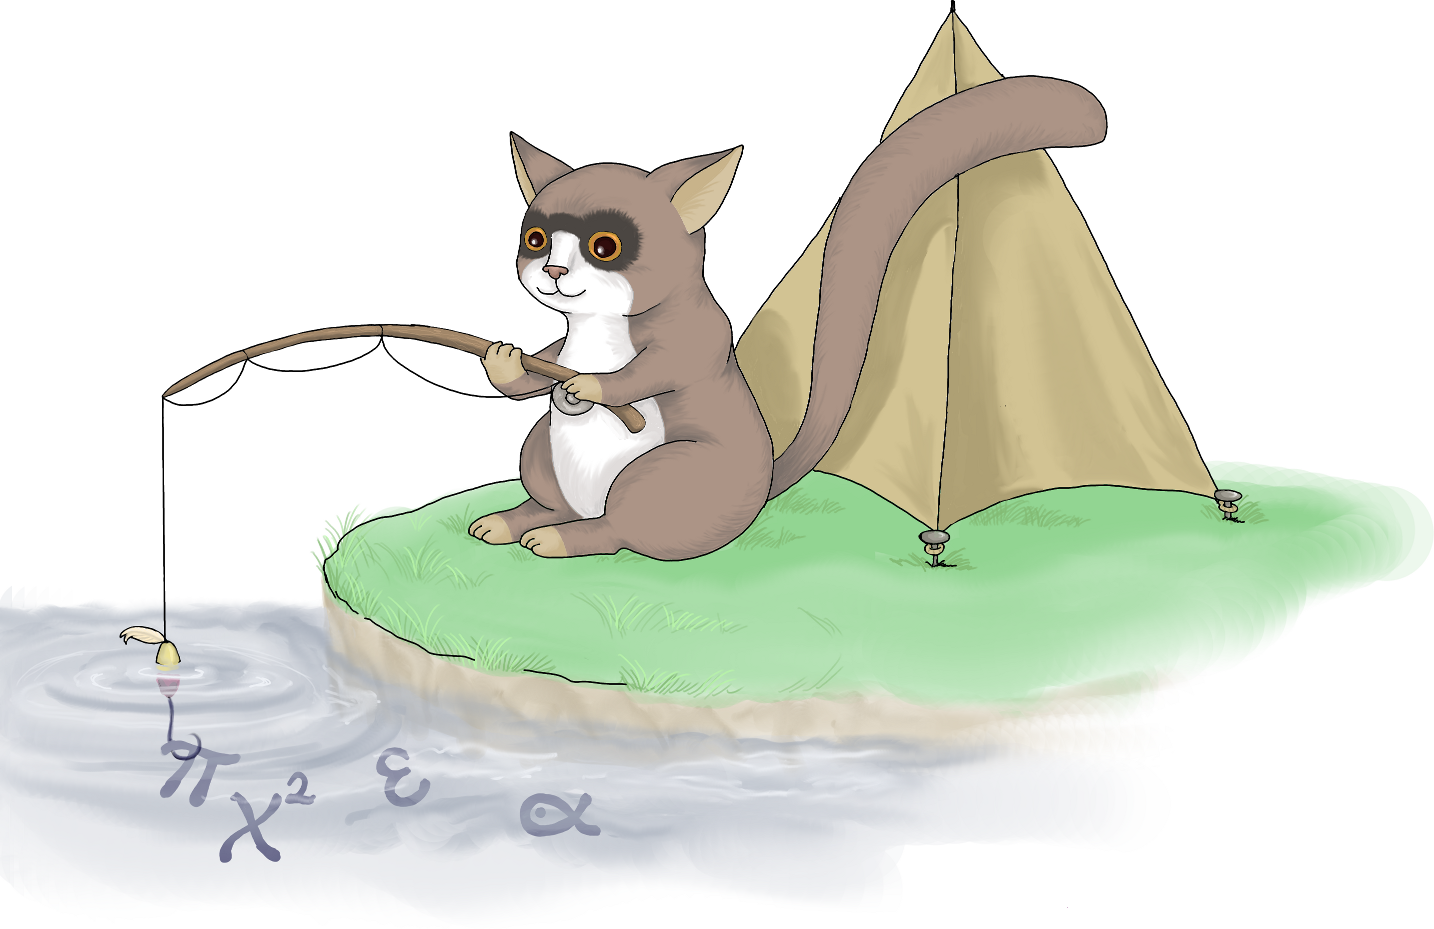
\includegraphics[scale=0.18]{campgregor}}}

\usepackage{framed}
\definecolor{shadecolor}{rgb}{.97,.97,.97}

\geometry{tmargin=1.5cm,bmargin=1.5cm,lmargin=2.5cm,rmargin=2.5cm}

\renewcommand{\gregor}{\put(13.2,-3.0){
\includegraphics[scale=0.18]{cover}}}
\begin{document}

\renewcommand{\betreff}{Mathecamp des Matheschülerzirkels Augsburg vom 22. bis
28. August}

\makeletterhead{}
\begin{picture}(0,0)
  \put(7.0,-19.0){%
    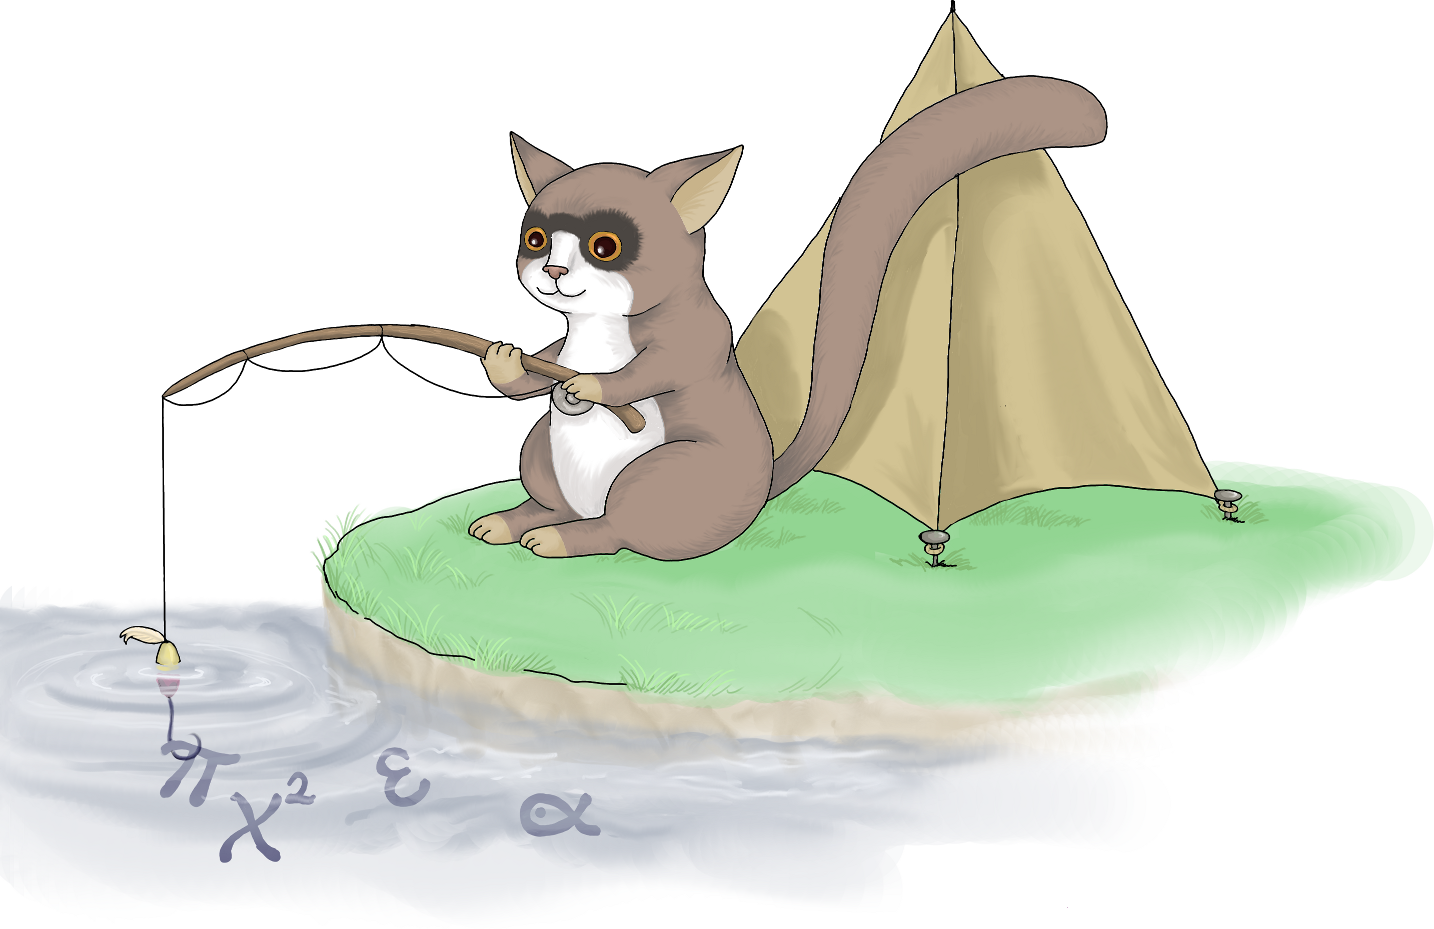
\includegraphics[scale=0.2]{campgregor}
  }
\end{picture}
\vspace{-2em}

Liebe Schülerinnen und Schüler, liebe Eltern,

wir laden euch herzlich zum zweiten Mathecamp des Matheschülerzirkels Augsburg
ein. Dort werden wir mit euch vielfältige mathematische Themen verstehen und die
Freizeit in den Ferien genießen. Darüber hinaus ist das Camp eine gute
Möglichkeit, Gleichgesinnte kennenzulernen und neue Freunde zu finden.
Nachdem es euch und uns letztes Jahr so viel Freude bereitet hat, haben wir das
Camp für dieses Jahr um zwei Tage verlängert.

\begin{tabbing}
  \hspace{2.2cm} \= \kill
  \textbf{Was?} \> Mathematik und Spaß in den Ferien \\[0.3em]
  \textbf{Wann?} \> 22. bis 28. August 2015 (Samstag bis Freitag) \\[0.3em]
  \textbf{Wo?} \> Bruder-Klaus-Heim in Violau, Schullandheim der Diözese
  Augsburg \\[0.3em]
  \textbf{Für wen?} \> \begin{minipage}[t]{\dimexpr\textwidth-2.3cm}
  Einzige Teilnahmevoraussetzung ist Spaß und Interesse an
  Mathematik.
  Jeder kann mitkommen, auch, wenn man nicht bei den Zirkeln
  mitgemacht hat.\end{minipage} \\[0.3em]
  \textbf{Kosten?} \> 230,-- \texteuro
\end{tabbing}

An jedem Tag werden vormittags zwei Arbeitsgruppen stattfinden. Dabei behandeln wir spannende
Bereiche der Mathematik, die in der Schule nicht thematisiert werden und die
wir auch nicht in den Präsenz- und Korrespondenzzirkeln gesehen haben.
Selbstverständlich gibt es für verschiedene Alters- und Vorkenntnisstufen angepasste Kurse
mit unterschiedlichen Themen und Schwierigkeiten, sodass immer für jeden
etwas dabei ist. Zusätzlich gibt es nachmittags weitere, optionale,
Arbeitsgruppen.

Daneben stehen Spiele- und Bastelstunden sowie die
Sternwarte des Heims auf dem Programm. Natürlich hoffen wir auf
schönes Wetter, damit wir auch die Tiere auf dem Gelände besuchen
und am Abend am Lagerfeuer grillen und Musik machen können.
Weiterhin stehen uns eine Pizzabäckerei, ein Volleyball- und ein
Fußballplatz zur Verfügung, sodass sicher niemandem langweilig
wird.
% Außerdem wird es zwei Vorträge von einer auswärtigen Mathematikerin und einem Mathematiker geben.

\vspace{\medskipamount}

\begin{minipage}{0.63\textwidth}
Wenn ihr teilnehmen möchtet, bittet eure Eltern das beiliegende Anmeldeformular
bis zum 1. Juni 2015 auszufüllen und an uns zurückzuschicken. Zusagen
verschicken wir nach Reihenfolge des Eingangsdatums.
\end{minipage}

\vspace{\medskipamount}

\begin{minipage}{0.4\textwidth}
Wenn ihr Freunde
habt, die Spaß an Mathe haben und ebenfalls gerne mit auf das
Camp fahren möchten, aber nicht an den Zirkeln beteiligt waren, so
können diese trotzdem gerne mitkommen.
\end{minipage}

\newpage

Getragen wird das Camp vom Mathematisch-Physikalischen Verein e.\,V. Das
Betreuer- und Organisationsteam um Sven Prüfer und Kathrin Helmsauer besteht
aus DoktorandInnen und MitarbeiterInnen des Instituts, die in ihrer Freizeit
ehrenamtlich interessierten Schülerinnen und Schülern Mathematik näherbringen
wollen. Alle Betreuer haben
bereits Erfahrungen in der Jugendarbeit und bei der Durch\-füh\-rung von
Sommercamps.

Wir bitten, den Betrag bis zum 8. Juni 2015 auf unser Konto zu überweisen.
In ihm sind die Kosten für An- und Abreise, Unterkunft, Verpflegung
(Vollpension) und Freizeitaktivitäten enthalten; wir Betreuer arbeiten
ehrenamtlich. Die Höhe der Eigenbeteiligung soll kein Teilnahmehindernis sein.
Familien, für die diese eine große finanzielle Belastung darstellt, bitten wir,
mit uns informal und formlos Kontakt aufzunehmen. Im Rahmen der finanziellen Möglichkeiten des
Vereins können wir gegebenenfalls auf den Beitrag verzichten.

\vspace{-0.7em}
\begin{tabbing}
  \qquad\quad \= Verwendungszweck:\, \= \kill
  \> Kontoinhaber: \> Mathematisch-Physikalischer Verein e.\,V. \\
  \> Konto-Nr.: \> 0810623223 \\
  \> BLZ: \> 72050000 (Stadtsparkasse Augsburg) \\
  \> IBAN: \> DE08720500000810623223 \\
  \> BIC: \> AUGSDE77 \\
  \> Betrag: \> 230,-- \texteuro{} bzw. 225,-- \texteuro, falls Bettwäsche
  mitgebracht wird \\
  \> Verwendungszweck: \> Mathecamp \emph{Vorname Nachname}
\end{tabbing}
\vspace{-0.7em}

Das Camp beginnt am 22. August zwischen 10:00 Uhr und 11:00 Uhr. Ihr könnt
entweder individuell zu dieser Zeit anreisen oder euch um 09:30 Uhr auf dem Campus der
Universität einfinden, um dann gemeinsam mit uns im Reisebus nach Violau zu fahren.
Die Abreise ist am 28. August ab 16:30 Uhr. Ihr könnt euch entweder von euren
Eltern abholen lassen oder mit uns zurück nach Augsburg fahren. Dort kommen wir
gegen 17:30 Uhr an der Universität an.

Wir schicken euch Ende Juli eine Übersicht mit
letzten Details und Kontaktdaten vor Ort. Bei Fragen stehen wir euch jederzeit
zur Verfügung. Bitte zögert nicht, uns dazu telefonisch unter 0821/598-5805
(Sven Prüfer) oder per Mail an \textsf{mathezirkel@math.uni-augsburg.de} zu kontaktieren.

Wir hoffen, dass wir
euch auf dem Mathecamp begrüßen dürfen und dass
ihr euch darauf genauso freut wie wir!

\vspace{2em}

Euer Team vom Mathezirkel

{\small Meru Alagalingam, Tim Baumann, Martin Baur, Ingo Blechschmidt, Philipp Düren,
Alexander Engel, Tim Dafler, Dominik Dirr, Lukas Graf, Kathrin Helmsauer, Prof. Dr. Marco Hien,
Christian Hübschmann, Jil Hümmer, Simon Kapfer, Sven Prüfer, PD Dr. Peter Quast,
Lisa Reischmann, Caren Schinko, Peter Uebele, Carina Willbold,
Stephanie Zapf}

\vfill

PS: Letztes Jahr konnten wir aufgrund einer großzügigen und einmaligen
finanziellen Unterstützung eines Lehrstuhls die Selbstbeteiligung deutlich
reduzieren. Da anderweitige Fördermittel diese Zuwendung nicht vollständig
ersetzen konnten, muss dieses Jahr die Eigenbeteiligung leider erheblich näher
an den anfallenden Kosten
liegen. Wenn Sie unsere Arbeit unterstützen
und dadurch auch zukünftig Veranstaltungen dieser Art ermöglichen möchten,
können Sie gerne einen höheren Beitrag überweisen. Als gemeinnütziger Verein
stellen wir dann eine Spendenbescheinigung über den zusätzlichen
Betrag aus.

\end{document}
